\documentclass[xcolor=x11names,compress]{beamer}
\usepackage[english]{babel}

%% General document %%%%%%%%%%%%%%%%%%%%%%%%%%%%%%%%%%

\usepackage{mathpazo}
\usepackage{graphicx}
\usepackage{tikz}
\usepackage{wrapfig}
\usepackage{hyperref}
\usepackage{fancybox,subcaption}
\usetikzlibrary{arrows}
\tikzstyle{block}=[draw opacity=0.7,line width=1.4cm]
\usetikzlibrary{decorations.fractals}
%%%%%%%%%%%%%%%%%%%%%%%%%%%%%%%%%%%%%%%%%%%%%%%%%%%%%%


%% Beamer Layout %%%%%%%%%%%%%%%%%%%%%%%%%%%%%%%%%%
\useoutertheme[subsection=false,shadow]{miniframes}
\useinnertheme{default}
\usefonttheme{serif}
\usepackage{palatino}

\setbeamerfont{title like}{shape=\scshape}
\setbeamerfont{frametitle}{shape=\scshape}

\setbeamercolor*{lower separation line head}{bg=DeepSkyBlue4} 
\setbeamercolor*{normal text}{fg=black,bg=white} 
\setbeamercolor*{alerted text}{fg=red} 
\setbeamercolor*{example text}{fg=black} 
\setbeamercolor*{structure}{fg=black}	%The color of title texts 
 
\setbeamercolor*{palette tertiary}{fg=black,bg=black!10} 
\setbeamercolor*{palette quaternary}{fg=black,bg=black!10} 


\newenvironment<>{problock}[1]{%
  \begin{actionenv}#2%
      \def\insertblocktitle{#1}%
      \par%
      \mode<presentation>{%
        \setbeamercolor{block title}{fg=white,bg=DeepSkyBlue4}
       \setbeamercolor{block body}{fg=black,bg=black!10}
       \setbeamercolor{itemize item}{fg=blue!20!black}
       \setbeamertemplate{itemize item}[triangle]
     }%
      \usebeamertemplate{block begin}}
    {\par\usebeamertemplate{block end}\end{actionenv}}


\useinnertheme[shadow=true]{rounded}
\usepackage{gnuplottex}
\renewcommand{\(}{\begin{columns}}
\renewcommand{\)}{\end{columns}}
\newcommand{\<}[1]{\begin{column}{#1}}
\renewcommand{\>}{\end{column}}
%%%%%%%%%%%%%%%%%%%%%%%%%%%%%%%%%%%%%%%%%%%%%%%%%%
\newcommand{\hlb}[1]{\textbf{\textcolor{DeepSkyBlue4}{#1}}}
\newcommand{\hl}[1]{\textcolor{blue}{#1}}
\newcommand{\lien}[2]{\mathcal{L}_{#1}^{#2}}
\newcommand{\lie}[1]{\mathcal{L}_{#1}}
\newcommand{\colv}[2]{\begin{pmatrix}#1\\#2\end{pmatrix}}
\newcommand{\colvt}[3]{\begin{pmatrix}#1\\#2\\#3\end{pmatrix}}
\newcommand{\bb}[1]{\textbf{#1}}
\newcommand{\mb}[1]{\mathbf{#1}}
\newcommand{\para}{\paragraph}
\newcommand{\subpara}{\subparagraph}
\newcommand{\abso}[1]{\left|#1\right|}


\usepackage[utf8]{inputenc}
%%%%%%%%%%%%%%%%% stuff for including svg images %%%%%%%%%%%%%
\newcommand{\executeiffilenewer}[3]{%
 \ifnum\pdfstrcmp{\pdffilemoddate{#1}}%
 {\pdffilemoddate{#2}}>0%
 {\immediate\write18{#3}}\fi%
}

\newcommand{\includesvg}[1]{%
 \executeiffilenewer{#1.svg}{#1.pdf}%
 {inkscape -z -D --file=#1.svg %
 --export-pdf=#1.pdf --export-latex}%
 \input{#1.pdf_tex}%
}








\begin{document}
\title{Investigating Piecewise Smooth Hybrid Systems}
\author{Debsankha Manik}

\begin{frame}
\titlepage
\end{frame}

\section{Introduction}
\begin{frame}{Hybrid systems}
These are systems described partly by differential equations and partly by 
maps: a \emph{hybrid} of continuous time and discrete time systems.  \\



\hlb{Examples:}
\begin{itemize}
\item A bell. 
\item A typewriter.  
\item Walking motion.  
\end{itemize}
\end{frame}

\begin{frame}{Mathematical Definition}
\begin{problock}{Piecewise smooth hybrid system}
A system described by a set of ODE's and a set of \bb{reset maps}:
\begin{align}
\label{def-hybrid}
\dot{x}&=F_i(x,\mu),~~\forall x\in S_i\\
x&\mapsto R_{ij}(x,\mu),~~\forall x\in\Sigma_{ij}=\bar{S_i}\cup\bar{S_j}
\end{align}

is called a piecewise smooth hybrid system if all the $R_i$'s, $F_i$'s as well 
as the associated flows $\varphi_i$'s are smooth in both $x$ and the parameter 
$\mu$ in the appropriate regimes.  
\end{problock}

\end{frame}


\begin{frame}{Example: Oscillator with hard impacts\\}
\begin{figure}[!hbp]
\caption{Hard impacting oscillator}
\label{fig-himp}
\begin{center}
\def\svgwidth{0.3\columnwidth}
\includesvg{hardcol}
\end{center}
\end{figure}

\begin{align}
\label{eq-hard_impact}
m\ddot{x}&=-\gamma \dot{x}-k_1x+G(t)&\mathrm{for}~~x<\sigma\\
(x,v)&\mapsto (x,-rv)&\mathrm{for}~~x=\sigma
\end{align}


$r$ is the coefficient of restitution, which is $1$ for perfectly 
elastic collisions.  
\end{frame}

\begin{frame}{Bifurcations in Hybrid Systems}
\hlb{Bifurcations} are \emph{qualitative} change in steady state system behaviour on a change of 
system parameters.  \\

\vspace{1em}
\pause{}
Bifurcations which are direct consequence of the switching  of the system dynamics
at the switching manifold are called \hlb{border collision bifurcations}.

\pause{}
\begin{tiny}
\begin{figure}
\begin{subfigure}{0.45\linewidth}
%\caption*{Before border collision: period 1}
\begin{center}
\def\svgwidth{0.9\linewidth}
\includesvg{pw-perdoub-bef}
\end{center}
\end{subfigure}%
$\to$
\begin{subfigure}{0.45\linewidth}
%\caption*{After border collision: period 2}
\begin{center}
\def\svgwidth{0.9\linewidth}
\includesvg{pw-perdoub-aft}
\end{center}
\end{subfigure}
\end{figure}
\end{tiny}
\end{frame}

\begin{frame}{Grazing bifurcation of limit cycles}
\begin{figure}[!htp]
\caption{Grazing orbit}
\label{fig-grazing-orbit}
\begin{center}
\def\svgwidth{0.7\columnwidth}
\includesvg{graz}
\end{center}
\end{figure}
\end{frame}

\section{The impact oscillator}
\begin{frame}
\begin{figure}[!hbp]
\caption{Hard impacting oscillator}
\label{fig-himp}
\begin{center}
\def\svgwidth{0.3\columnwidth}
\includesvg{hardcol}
\end{center}
\end{figure}

\begin{align}
\label{eq-hard_impact}
m\ddot{x}&=-\gamma \dot{x}-\omega_0^2x+F\cos{\omega 
t}&\mathrm{for}~~x<\sigma\\
(x,v)&\mapsto (x,-rv)&\mathrm{for}~~x=\sigma
\end{align}

\end{frame}

\begin{frame}
If we forget the boundary for a moment, the equation of motion is a non-homogeneous 
ODE.  As usual, its solution is a sum total of a \emph{homogeneous solution} 
and a \emph{particular solution}:
\begin{align}
\label{eq-shm-sol}
x(t)&=x_p(t)+x_h(t)\\
x_p(t)&=\frac{F/m}{\sqrt{(\omega_0^2-\omega^2)^2+\omega^2\gamma^2}}cos(\omega t+tan^{-1}\frac{\omega \gamma}{\omega^2-\omega_0^2})\\
x_h(t)&=\frac{e^{-\gamma t/2}}{\omega_g}\left\{(\omega_g\cos{\omega_gt}+\frac{\gamma}{2}\sin{\omega_gt})x(0) + (\sin{\omega_gt})v(0) \right\}\\
\omega_g&=\sqrt{\omega_0^2-\frac{\gamma^2}{4}}
\end{align}

\end{frame}

\begin{frame}{A few possible trajectories}

\begin{figure}
\begin{center}
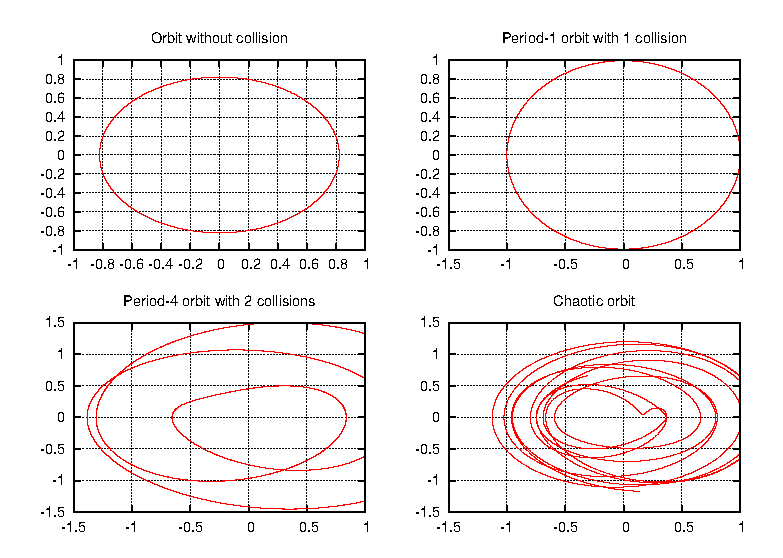
\includegraphics[width=\columnwidth]{many-orbs}
\end{center}
\end{figure}

\end{frame}

\begin{frame}{Stroboscopic Poincaré map}
\begin{figure}
\begin{center}
\def\svgwidth{0.9\columnwidth}
\includesvg{strobo}
\end{center}
\end{figure}
\end{frame}

\section{Vanishing chaos}

\begin{frame}
Kundu and Banerjee \cite{banerjee-kundu-soft,banerjee-kundu-hard} investigated 
the grazing bifurcations in this system by deriving an approximate analytical expression 
for the stroboscopic  Poincaré map near grazing. \\


\hlb{Their results:}
\begin{itemize}
\item Unless $n=\frac{2\omega_g}{\omega_{forcing}}\in \mathbb{N}$, chaos 
immediately follows grazing of the steady state orbit.  
\item If $n\in\mathbb{N}$, no chaos after grazing.  
\end{itemize}
\hlb{Experimental data:}
\begin{itemize}
\item Chaos vanishes not only \emph{at} $n\in\mathbb{N}$, but at small 
neighbourhoods around each $n\in\mathbb{N}$
\end{itemize}
\end{frame}

\begin{frame}

\begin{tiny}
\begin{figure}
\begin{subfigure}{0.5\linewidth}
\begin{center}
\caption*{Bifurcation digram for $n=2.2$}
\label{fig-bif-int}
\def\svgwidth{\columnwidth}
\includesvg{bifurcation-ni}
\end{center}
\end{subfigure}%
\begin{subfigure}{0.5\linewidth}
\begin{center}
\caption*{Bifurcation diagram for $n=2$}
\def\svgwidth{\columnwidth}
\label{fig-bif-nonint}
\includesvg{bifurcation-n-2}
\end{center}
\end{subfigure}
\end{figure}
\end{tiny}
\end{frame}

\begin{frame}{Numerical computation of orbits}
The bifurcation diagrams suggest that for $n\in\mathbb{N}$, a stable period-1 
orbit emerges right after grazing, unlike non-integer $n$ values.  

We used a method devised by Ma et al.\cite{ma-nraphson} for checking if that 
indeed is the case.  

\begin{tiny}
\begin{figure}[!hbp]
\begin{center}
\def\svgwidth{0.6\columnwidth}
\includesvg{num-sol}
\end{center}
\end{figure}
\end{tiny}
\end{frame}

\begin{frame}
Define $y=(x_0,v_0,x_c,v_c,\tau)$

Then we get a system of equations $\mb{G}(y)=\mb{0}$ where:
\begin{align*}
G_{1,2}(y)=\vec{x_c}-\varphi(\tau,0,\vec{x_0})&=0\\
G_{3,4}(y)=\vec{x_0}-\varphi(2T,\tau,\vec{x_c})&=0\\
G_5(y)=x_1-\sigma&=0
\end{align*}

Since this is a set of 5 equations in 5 unknowns, we can solve the equation $G(y)=0$ using Newton-Raphson method:
\[
y_{n+1}=y_n+J(y)^{-1}G(y)
\]
\end{frame}

\begin{frame}
\begin{tiny}
\begin{figure}
\begin{center}
\def\svgwidth{\columnwidth}
\includesvg{num-eigs}
\end{center}
\end{figure}
\end{tiny}
\end{frame}

\section{Impact map}
\begin{frame}{Analytical approach}
\begin{figure}[!htp]
\centering
\caption{Impact map in case of $PnC1$ orbit}
\label{fig-impmap-dia}
\def\svgwidth{0.4\columnwidth}
\includesvg{impactmap}
\end{figure}

\begin{align}
\label{def-mi}
M_I:\colv{x}{v}&\mapsto M(mT)\colv{x}{-v\pm2\omega \sqrt{A^2-(\sigma-x})^2}
\end{align}

\begin{eqnarray}
\label{def-huge-M-matrix}
M(t)=\frac{e^{-\gamma t/2}}{\omega_g}
\begin{pmatrix}
\omega_g\cos{\omega_g t}+\frac{\gamma}{2}\sin{\omega_g t} & \sin{\omega_g t}\\
-k\sin{\omega_g t} & \omega_g\cos{\omega_g t}-\frac{\gamma}{2}\sin{\omega_g t}
\end{pmatrix}
\end{eqnarray}
\end{frame}

\begin{frame}{The fixed points and the Jacobian}
\hlb{Fixed points}
\begin{align}
\label{fp-solution}
x^*&=\frac{\sigma\pm\sqrt{\sigma^2-(\alpha^2+1)(\sigma^2-A^2)}}{\alpha^2+1}\\
v^*&=\frac{(d-ad+bc)x^*}{b}\\
M(mT)&=
\begin{pmatrix}
a & b\\
c & d
\end{pmatrix}\\
\alpha&=\frac{(a-d+ad-bc-1)}{2b\omega}
\end{align}

\hlb{The Jacobian}
\begin{align}
\label{eq-jac-mi}
J(x,v)&=M(mT)
\begin{pmatrix}
1 & 0\\
-v\pm2\omega \frac{\sigma-x}{\sqrt{A^2-(\sigma-x})^2} & -1
\end{pmatrix}
\end{align}

\end{frame}

\begin{frame}
\begin{tiny}
\begin{figure}[!htp]
\begin{center}
\caption{Eigenvalues of J at fixed points Vs.  $F$ for $n=2.01,2.1,2.2$}
\def\svgwidth{0.8\textwidth}
\includesvg{many-n}
\end{center}
\end{figure}
\end{tiny}
\end{frame}

\begin{frame}
\begin{tiny}
\begin{figure}[!htp]
\begin{center}
\caption{Eigenvalues of J at fixed points at grazing Vs. $n$}
\label{fig-eigs-n}
\def\svgwidth{0.8\textwidth}
\includesvg{probing_n_2pi}
\end{center}
\end{figure}
\end{tiny}
\end{frame}

\section{Long transients}
\begin{frame}
\begin{figure}[!htb]
\caption{Average transient lifetime Vs.  $F$ in the hard impacting oscillator}
\label{fig-tvsf}
\begin{center}
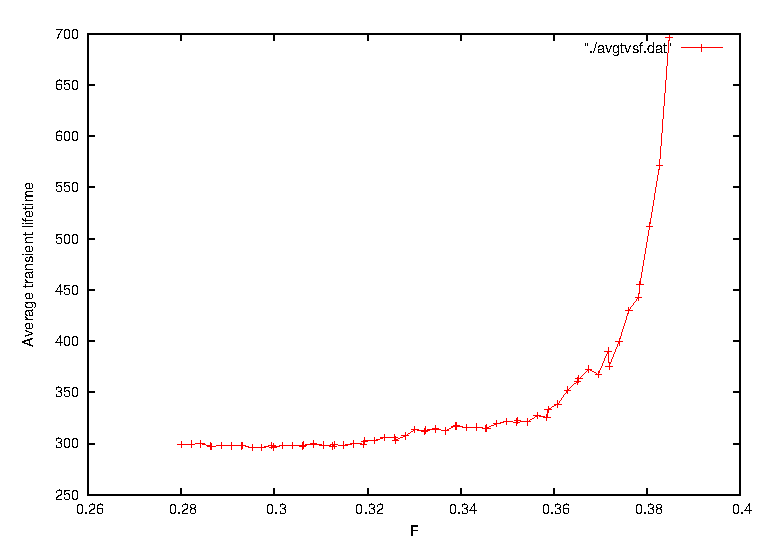
\includegraphics[width=0.9\columnwidth]{avgtauvsf-wofit}
\end{center}
\end{figure}
\end{frame}
\begin{frame}
\begin{figure}[!htp]
\caption{Average transient lifetime Vs.  $\gamma$ in the hard impacting oscillator}
\label{fig-tvsg}
\begin{center}
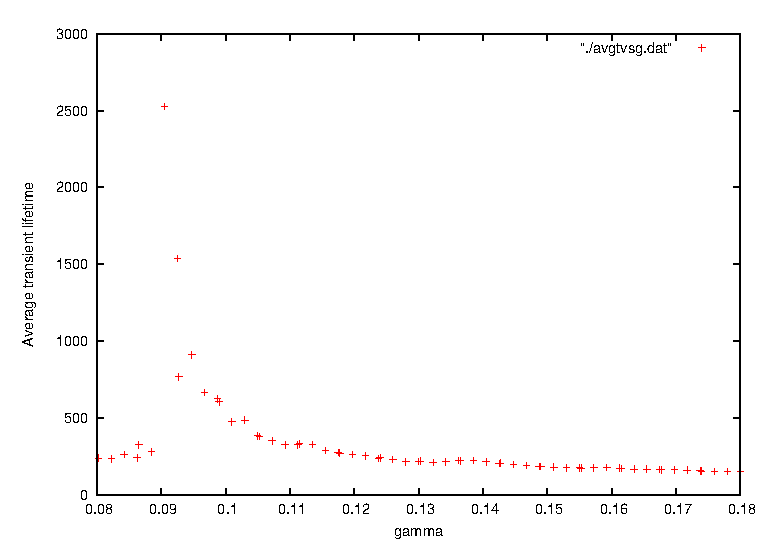
\includegraphics[width=0.9\columnwidth]{avgtauvsg-wofit}
\end{center}
\end{figure}
\end{frame}

\begin{frame}
Grebogi et al.\cite{grebogi-transient} predicted:

\begin{align}
\label{form-transient-life}
\tau\propto |\rho-\rho_c|^{-n}
\end{align}

\pause{}
These long lived transients are \emph{artefacts 
of the nonlinearity} due to the impacts. \\
Without impacts,
transient  decays as
\begin{align}
x_h(t)&=\frac{e^{-\gamma t/2}}{\omega_g}\left\{(\omega_g\cos{\omega_gt}+\frac{\gamma}{2}\sin{\omega_gt})x_0 + (\sin{\omega_gt})v_0 \right\}
\end{align}
\pause{}

In that case, $\tau$ would vary inversely with 
$\gamma$ and would not depend on $F$ at all.\\

\pause{}
Therefore, we need to concentrate on the impacts.  
\end{frame}

\begin{frame}
Consider an initial condition:
\begin{align*}
\vec{x_p}(0)&=(-A,0)\\
\vec{x_h}(0)&=(x_0,v_0)
\end{align*}

Where $A=\frac{F/m}{\sqrt{(\omega_0^2-\omega^2)^2+\omega^2\gamma^2}}$

\pause{}
Starting from this point, the solution till the next collision is, as per \eqref{eq-shm-sol}:

\begin{align*}
x(t)&=-A\cos{\omega t}+\frac{e^{-\gamma t/2}}{\omega_g}\left\{(\omega_g\cos{\omega_gt}+\frac{\gamma}{2}\sin{\omega_gt})x_0 + (\sin{\omega_gt})v_0 \right\}\\
&=-A\cos{\omega t}+e^{-\gamma t/2}B\cos{\left(\omega_g t+C\right)}\\
C&=-tan^{-1}\frac{\frac{\gamma}{2\omega_g}x_0+\frac{v_0}{\omega_g}}{x_0}\\
B&=\sqrt{x_0^2+\left(\frac{\gamma}{2\omega_g}x_0+\frac{v_0}{\omega_g}\right)^2}
\end{align*}
\end{frame}

\begin{frame}
\begin{figure}[!htb]
\begin{center}
\caption{An envelope of \eqref{eq-shm-sol} for $\omega_g\approx \omega$}
\label{fig-envelope-beats}
\def\svgwidth{0.9\columnwidth}
\includesvg{envc1}
\end{center}
\end{figure}
\end{frame}

\begin{frame}
\begin{figure}[!htb]
\begin{center}
\caption{An envelope of \eqref{eq-shm-sol} for $\omega_g\gg\omega$}
\def\svgwidth{0.9\columnwidth}
\includesvg{envc2}
\end{center}
\end{figure}
\end{frame}

\begin{frame}
Measuring how ``collision-prone'' the system is for a certain fixed parameter value:
\begin{enumerate}
\item Consider a large number of initial conditions $(x_0,v_0)\in \mathbb{R}^2$.  
\pause{}
\item Using the envelope, predict if there will be 
any future collision or not if the system starts from that initial condition.  
\pause{}
\item Points for which there is no further collision should form a closed area 
in the whole space $\mu_{xv}$  
\pause{}
\item See how this area shrinks as we approach grazing.  
\end{enumerate}

\pause{}
\begin{align}
\label{mu-analytical}
\mu_{xv}&\approx2\omega_g\int_{-\chi}^{max\{\chi,\sigma\}} \sqrt{\chi^2-x^2}dx\\
\chi&=(\sigma-A)e^{\gamma t_c/2}
\end{align}

We hope $\tau\propto\frac{1}{\mu_{xv}}$
\end{frame}

\begin{frame}
\begin{figure}
\begin{subfigure}{0.5\linewidth}
\begin{center}
\caption*{$\mu_{xv}$ vs.  $F$}
\label{fig-scanf}
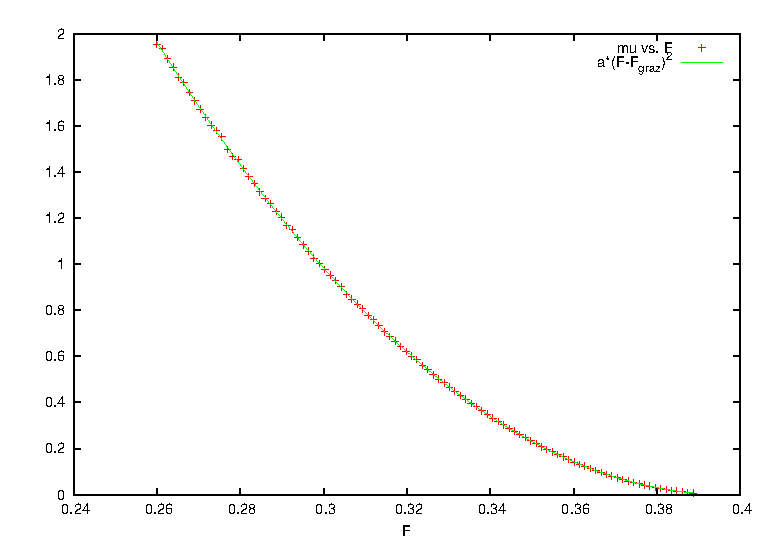
\includegraphics[width=\columnwidth]{scanf}
\end{center}
\end{subfigure}%
\begin{subfigure}{0.5\linewidth}
\begin{center}
\caption*{$\mu_{xv}$ vs.  $\gamma$}
\label{fig-scang}
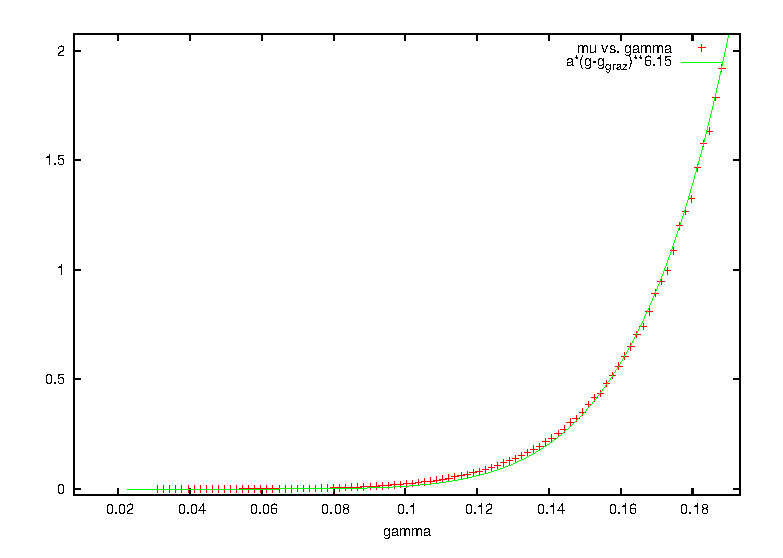
\includegraphics[width=\columnwidth]{scang}
\end{center}
\end{subfigure}
\end{figure}
\end{frame}

\begin{frame}
\begin{tiny}
\begin{figure}
\begin{subfigure}{0.5\linewidth}
\begin{center}
\caption*{$\mu_{xv}$ vs.  $F$}
\def\svgwidth{\columnwidth}
\includesvg{tauvsf}
\label{fig-scanf}
\end{center}
\end{subfigure}%
\begin{subfigure}{0.5\linewidth}
\begin{center}
\caption*{$\mu_{xv}$ vs.  $\gamma$}
\def\svgwidth{\columnwidth}
\includesvg{tauvsg}
\label{fig-scang}
\end{center}
\end{subfigure}
\end{figure}
\end{tiny}
\end{frame}








\nocite{*}
\bibliography{thesis}{}
\bibliographystyle{plain}

\end{document}
